\documentclass{standalone}

\usepackage{amsmath}
\usepackage{tikz}
\usetikzlibrary{arrows.meta, positioning, calc, patterns}

\renewcommand{\familydefault}{\rmdefault}
\usepackage{dsfont}
\usepackage[T1]{fontenc}
\usepackage{lmodern}

\begin{document}

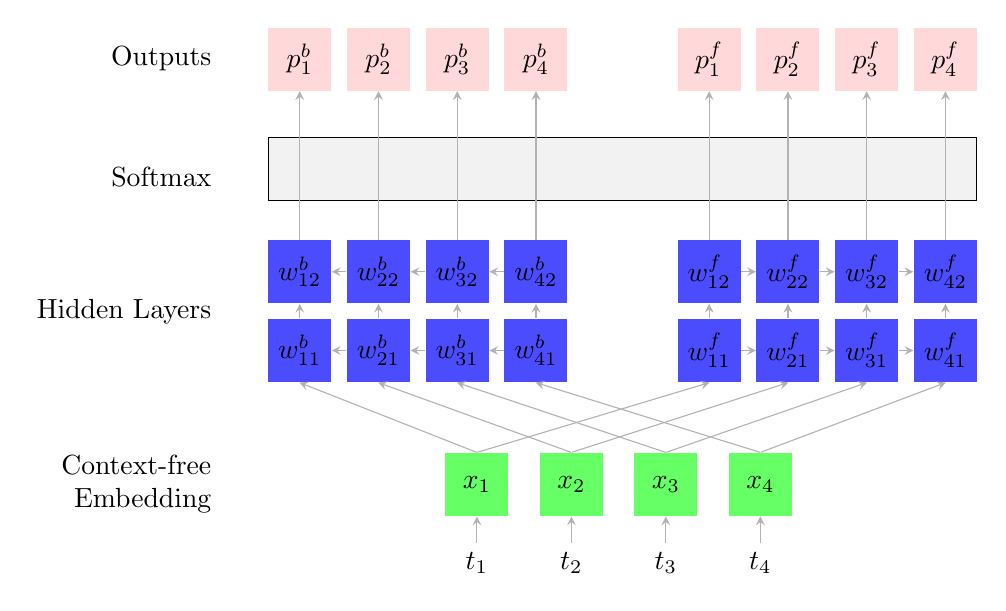
\begin{tikzpicture}[
    >=stealth,
    embed/.style={rectangle, fill=green!60, minimum size=8mm},
    hidden/.style={rectangle, fill=blue!70, minimum size=8mm},
    output/.style={rectangle, fill=pink!60, minimum size=8mm},
    conn/.style={gray!60,->,thin}
]

% -------- Spacing controls --------
\def\gap{1}      % spacing within group
\def\biggap{2.2}   % spacing between b and f groups

% -------- X positions --------
\def\xA{0}
\def\xB{\xA+\gap}
\def\xC{\xB+\gap}
\def\xD{\xC+\gap}

\def\xE{\xD+\biggap}
\def\xF{\xE+\gap}
\def\xG{\xF+\gap}
\def\xH{\xG+\gap}

% embedding centers
\def\xstart{2.25}
\def\xgap{1.2}

\pgfmathsetmacro{\xeA}{\xstart}
\pgfmathsetmacro{\xeB}{\xstart + \xgap}
\pgfmathsetmacro{\xeC}{\xstart + 2*\xgap}
\pgfmathsetmacro{\xeD}{\xstart + 3*\xgap}

% -------- Y levels --------
\def\yembed{0}
\def\yhidden{2.2}
\def\ysoft{3.9}
\def\yout{5.4}

% -------- Left labels (moved left for space) --------
\node[left] at (-1,\yout) {Outputs};
\node[left] at (-1,\ysoft) {Softmax};
\node[left] at (-1,\yhidden) {Hidden Layers};
\node[left, align=right] at (-1,\yembed) {Context-free\\Embedding};

% -------- Embeddings (more spaced) --------
% embeddings
\node[embed] (x1) at (\xeA,\yembed) {$x_1$};
\node[embed] (x2) at (\xeB,\yembed) {$x_2$};
\node[embed] (x3) at (\xeC,\yembed) {$x_3$};
\node[embed] (x4) at (\xeD,\yembed) {$x_4$};

% tokens (directly below)
\node (t1) at (\xeA,\yembed-1.0) {$t_1$};
\node (t2) at (\xeB,\yembed-1.0) {$t_2$};
\node (t3) at (\xeC,\yembed-1.0) {$t_3$};
\node (t4) at (\xeD,\yembed-1.0) {$t_4$};

% vertical arrows
\draw[conn] (t1.north) -- (x1.south);
\draw[conn] (t2.north) -- (x2.south);
\draw[conn] (t3.north) -- (x3.south);
\draw[conn] (t4.north) -- (x4.south);

% -------- Hidden layer --------

% backward
\foreach \x/\i in {\xA/1,\xB/2,\xC/3,\xD/4} {
    \node[hidden] (btop\i) at (\x,\yhidden+0.5) {$w^b_{\i 2}$};
    \node[hidden] (bbot\i) at (\x,\yhidden-0.5) {$w^b_{\i 1}$};
}

% forward
\foreach \x/\i in {\xE/1,\xF/2,\xG/3,\xH/4} {
    \node[hidden] (ftop\i) at (\x,\yhidden+0.5) {$w^f_{\i 2}$};
    \node[hidden] (fbot\i) at (\x,\yhidden-0.5) {$w^f_{\i 1}$};
}

% -------- Softmax (centered + wider) --------
\draw[fill=gray!10] (\xA-0.4,\ysoft-0.3) rectangle (\xH+0.4,\ysoft+0.5);

% -------- Outputs --------

% backward outputs
\node[output] (pb1) at (\xA,\yout) {$p^b_1$};
\node[output] (pb2) at (\xB,\yout) {$p^b_2$};
\node[output] (pb3) at (\xC,\yout) {$p^b_3$};
\node[output] (pb4) at (\xD,\yout) {$p^b_4$};

% forward outputs
\node[output] (pf1) at (\xE,\yout) {$p^f_1$};
\node[output] (pf2) at (\xF,\yout) {$p^f_2$};
\node[output] (pf3) at (\xG,\yout) {$p^f_3$};
\node[output] (pf4) at (\xH,\yout) {$p^f_4$};

% -------- x → hidden (clean, parallel, border-to-border) --------

\def\offset{0.12}

% x1
\draw[conn] ([xshift=-\offset]x1.north) -- ([xshift=-\offset]bbot1.south);
\draw[conn] ([xshift=\offset]x1.north) -- ([xshift=\offset]fbot1.south);

% x2
\draw[conn] ([xshift=-\offset]x2.north) -- ([xshift=-\offset]bbot2.south);
\draw[conn] ([xshift=\offset]x2.north) -- ([xshift=\offset]fbot2.south);

% x3
\draw[conn] ([xshift=-\offset]x3.north) -- ([xshift=-\offset]bbot3.south);
\draw[conn] ([xshift=\offset]x3.north) -- ([xshift=\offset]fbot3.south);

% x4
\draw[conn] ([xshift=-\offset]x4.north) -- ([xshift=-\offset]bbot4.south);
\draw[conn] ([xshift=\offset]x4.north) -- ([xshift=\offset]fbot4.south);

% -------- Hidden (top) → Output --------

% backward outputs
\draw[conn] (btop1.north) -- (pb1.south);
\draw[conn] (btop2.north) -- (pb2.south);
\draw[conn] (btop3.north) -- (pb3.south);
\draw[conn] (btop4.north) -- (pb4.south);

% forward outputs
\draw[conn] (ftop1.north) -- (pf1.south);
\draw[conn] (ftop2.north) -- (pf2.south);
\draw[conn] (ftop3.north) -- (pf3.south);
\draw[conn] (ftop4.north) -- (pf4.south);

% -------- Vertical (layer 1 → layer 2) --------

% backward
\foreach \i in {1,2,3,4} {
    \draw[conn] (bbot\i.north) -- (btop\i.south);
}

% forward
\foreach \i in {1,2,3,4} {
    \draw[conn] (fbot\i.north) -- (ftop\i.south);
}

% -------- Backward (right → left) --------
\foreach \i/\j in {2/1,3/2,4/3} {
    \draw[conn] (bbot\i.west) -- (bbot\j.east);
    \draw[conn] (btop\i.west) -- (btop\j.east);
}

% -------- Forward (left → right) --------
\foreach \i/\j in {1/2,2/3,3/4} {
    \draw[conn] (fbot\i.east) -- (fbot\j.west);
    \draw[conn] (ftop\i.east) -- (ftop\j.west);
}

\end{tikzpicture}
\hspace{1cm}
\end{document}